\section{Motivation and Vision}\label{Motivation-and-Vision}

MySQL is an easy relational database to get started with.
It's easy to setup and has a short learning curve.
However, as your system starts to scale, it begins to run out of steam.
This is mainly because it's non-trivial to shard a MySQL database after the fact.
Among other problems, the growing number of connections also becomes an
unbearable overhead.

On the other end of the spectrum, there are NoSQL databases.
However, they suffer from problems that mainly stem from the fact that they're new.
Those who have adopted them have struggled with the lack of secondary indexes,
table joins and transactions.

Vitess tries to bring the best of both worlds by trading off
some of MySQL's consistency features in order to achieve the
kind of scalability that NoSQL databases provide.

\subsubsection{Priorities}\hypertarget{priorities}{}\label{priorities}

\begin{itemize}
\item \emph{Scalability}: This is achieved by replication and sharding.
\item \emph{Efficiency}: This is achieved by a proxy server (vttablet) that mediates
all queries and connections.
It also utilizes a more efficient rowcache to short-cut some of the queries.
This effectively increases a typical MySQL's serving capacity.
\item \emph{Manageability}: As soon as you add replication and sharding that span
across multiple data centers, the number of servers spirals out of control.
Vitess provides a set of tools backed by a \index{lockserver}{\textbf{lockserver}} (zookeeper) to
track and administer them.
\item \emph{Simplicity}: As the complexity grows, it's important to hide this
from the application.
The vtgate servers give you a unified view of the fleet that makes
it feel like you're just interacting with one database.
\end{itemize}

\subsubsection{Trade-offs}\hypertarget{trade-offs}{}\label{trade-offs}

Scalability and availability require some trade-offs:
\begin{itemize}
\item  \emph{Consistency}: In a typical web application, not all reads have to be
fully consistent.

Vitess lets you specify the kind of consistency you want on your read.
It's generally recommended that you use replica reads as they're easier to scale.
You can always request for master reads if you want up-to-date data.
You can also additionally perform 'for update' reads that ensure that
a row will not change until you've committed your changes.
\item  \emph{Transactions}: Relational transactions are prohibitively expensive
across distributed systems.
Vitess eases this constraint and guarantees transactional integrity
'per keyspace id', which is restricted to one shard.
Heuristically, this tends to cover most of an application's transactions.
For the few cases that don't, you can sequence your changes in such a way
that the system looks consistent even if a distributed transaction fails
in the middle.
\item  \emph{Latency}: There is some negligible latency introduced by the proxy servers.
However, they make up for the fact that you can extract more throughput from
MySQL than you would otherwise be able to without them.
\end{itemize}

\subsubsection{Preserved MySQL features}\hypertarget{preserved-mysql-features}{}\label{preserved-mysql-features}

Since the underlying storage layer is still MySQL, we still get to preserve
its other important features:
\begin{itemize}
\item  \emph{Indexes}: You can create secondary indexes on your tables. This allows you
to efficiently query rows using more than one key.
\item  \emph{Joins}:  MySQL allows you to split one-to-many and many-to-many relational data
into separate tables, and lets you join them on demand.
\end{itemize}
This flexibility generally results in more efficient storage as each piece of
data is stored only once, and fetched only if needed.

\subsubsection{The Vitess spectrum}\hypertarget{the-vitess-spectrum}{}\label{the-vitess-spectrum}

The following diagram illustrates where vitess fits in the spectrum of storage solutions:

\begin{figure}[H]
\caption{Vitess Spectrum}
\label{fig:Vitess Spectrum}
\begin{center}
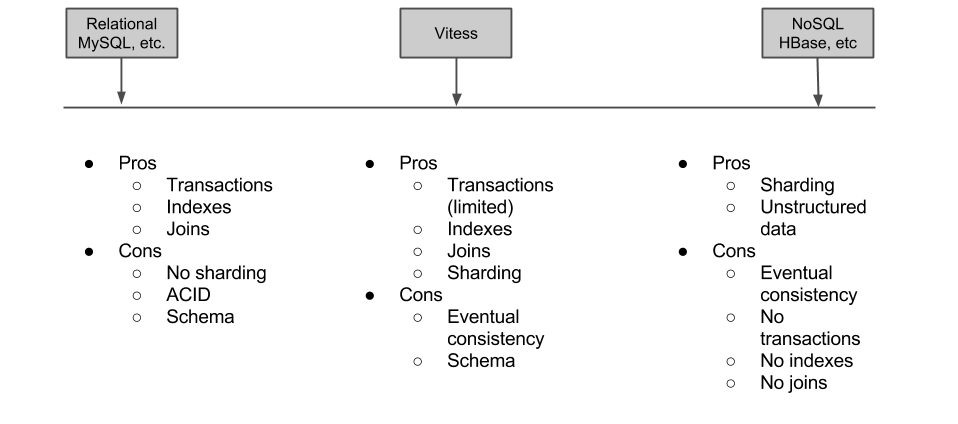
\includegraphics[scale=0.65]{VitessSpectrum.pdf}
\end{center}
\end{figure}




